\documentclass[12pt, titlepage]{article}

\usepackage{fullpage}
\usepackage[round]{natbib}
\usepackage{multirow}
\usepackage{booktabs}
\usepackage{tabularx}
\usepackage{graphicx}
\usepackage{float}
\usepackage{hyperref}
\usepackage{amsfonts}
\restylefloat{table}
\usepackage{ amssymb }

\hypersetup{
    colorlinks,
    citecolor=blue,
    filecolor=black,
    linkcolor=red,
    urlcolor=blue
}


%% Comments

\usepackage{color}

\newif\ifcomments\commentstrue %displays comments
%\newif\ifcomments\commentsfalse %so that comments do not display

\ifcomments
\newcommand{\authornote}[3]{\textcolor{#1}{[#3 ---#2]}}
\newcommand{\todo}[1]{\textcolor{red}{[TODO: #1]}}
\else
\newcommand{\authornote}[3]{}
\newcommand{\todo}[1]{}
\fi

\newcommand{\wss}[1]{\authornote{blue}{SS}{#1}} 
\newcommand{\plt}[1]{\authornote{magenta}{TPLT}{#1}} %For explanation of the template
\newcommand{\an}[1]{\authornote{cyan}{Author}{#1}}

%% Common Parts

\newcommand{\progname}{SE 4G06} % PUT YOUR PROGRAM NAME HERE
\newcommand{\authname}{Team \#6, Board Gamers
\\ Ilao Michael, ilaom
\\ Bedi Hargun, bedih
\\ Dang Jeffrey, dangj12
\\ Ada Jonah, karaatan
\\ Mai Tianzheng, mait6} % AUTHOR NAMES                  

\usepackage{hyperref}
    \hypersetup{colorlinks=true, linkcolor=blue, citecolor=blue, filecolor=blue,
                urlcolor=blue, unicode=false}
    \urlstyle{same}
                                


\newcounter{assumpnum}
\newcommand{\atheassumpnum}{P\theassumpnum}
\newcommand{\pref}[1]{P\ref{#1}}

\newcounter{acnum}
\newcommand{\actheacnum}{AC\theacnum}
\newcommand{\acref}[1]{AC\ref{#1}}

\newcounter{ucnum}
\newcommand{\uctheucnum}{UC\theucnum}
\newcommand{\uref}[1]{UC\ref{#1}}

\newcounter{mnum}
\newcommand{\mthemnum}{M\themnum}
\newcommand{\mref}[1]{M\ref{#1}}

\begin{document}
\title{Module Guide for SE 4G06 \\ An AI-based Approach to Designing Board Games} 
\author{\authname{}}
\date{\today}

\maketitle

\pagenumbering{roman}

\section{Revision History}

\begin{tabularx}{\textwidth}{p{3cm}p{2cm}X}
\toprule {\bf Date} & {\bf Version} & {\bf Notes}\\
\midrule
Date 1 & 1.0 & Notes\\
Date 2 & 1.1 & Notes\\
\bottomrule
\end{tabularx}

\newpage

\section{Reference Material}

This section records information for easy reference.

\subsection{Abbreviations and Acronyms}

\renewcommand{\arraystretch}{1.2}
\begin{tabular}{l l} 
  \toprule		
  \textbf{symbol} & \textbf{description}\\
  \midrule 
  AI & Artifical Intellegence \\
  GE & Game Engine\\
  DV & Data Visualizer \\
  M & Module \\
  MG & Module Guide \\
  OS & Operating System \\
  R & Requirement\\
  SC & Scientific Computing \\
  SRS & Software Requirements Specification\\
  \progname & Explanation of program name\\
  UC & Unlikely Change \\
  \bottomrule
\end{tabular}\\
\subsection{Guideline}
This Design Document, \href{https://gitlab.cas.mcmaster.ca/courses/capstone/-/blob/main/SamplesOfStudentWork/Design/Capstone%20Intelligence%20-%20System%20Design.pdf}{Capstone Intelligence} was used as a template and guideline for this document.
\newpage

\tableofcontents

\listoftables

\listoffigures

\newpage

\pagenumbering{arabic}

\section{Purpose}
\subsection{System Purpose} 
The purpose of the system is to simulate the board game An Age Contrived from Bellow Intent's using an AI-based game simulation engine. This system will help identify pitfall's in game mechanics and imbalances in the game's scoring system. The system will also be used to view decisions, scoring and other game state information through various plots, graphs and charts.
The system will be used by Game Designers of An Age Contrived to help balance their game as well as AI Research Professors to further understand and develop AI-based game engines.
\subsection{Document Purpose}
The purpose of this document is to decompose the system into different modules, to show the module and system architecture and provide justifications for each module. This will serve as a guideline for development of the system.

\section{Scope}
The system is to be used by game designers when creating and balancing their board games and AI researchers 
\subsection{Assumptions}
\begin{itemize}

\item[A\refstepcounter{assumpnum}\theassumpnum \label{A_Reward_Function}:]
  The game to be analyzed will have a clear reward function that AI Agent can optimize its learning towards.
  
\item[A\refstepcounter{assumpnum}\theassumpnum \label{A_End_Condition}:]
  The game to be analyzed will have a clear win condition where the game ends.\\ 
  \textbf{Rationale}: It shouldn't be an open-ended, infinite game where the goal is to just increase your score but rather there should be a specific condition(s) that players are playing towards to win and end the game. Otherwise, AI agents won't be able to find the optimal actions to win the game but rather keep outputting sub-optimal decisions which will have little to no value for game design improvements.
  
\item[A\refstepcounter{assumpnum}\theassumpnum \label{A_Representable}:]
  The game to be analyzed will have concrete rules that a computer can represent and enforce.\\
  \textbf{Rationale}: If the game cannot be simulated digitally, then AI Agent cannot be trained on the game and the system wouldn't be able to generate any meaningful data to aid the game design process.

\end{itemize}
\section{Project Overview}
\subsection{Normal Operation}
This project will be used by board game designers to rapid prototype their development of the game rules and game metrics. Board game designers will be able to evaluate the balance of their game in terms if there exists an always winning sequence of moves that are not intended to be that strong to achieve the win condition in their game. Simulating many games through AI players will save a large amount of time in testing by analyzing the moves and winning sequences of the large data set of games they will generate.
\subsection{Behaviour Overview}
The system is designed on a command pattern architecture. When the simulation is run, AI Agents are able to choose a selection of moves in. After a game move is chosen, the game engine will accept and change its state based on the move given. This will feedback on where the game engine will give the game state back to the AI Agents, which they can choose another action after receiving the game state. This will repeat until the end of the game is reached.  

\newpage
\subsection{Module Hierarchy}
\begin{table}[h!]
\centering
\begin{tabular}{p{0.1\textwidth} p{0.2\textwidth} p{0.6\textwidth}}
\toprule
\textbf{Module Type} & \textbf{Module Name} & \textbf{Module Description}\\
\midrule
AI & \multirow{1}{0.3\textwidth}{AI Agent Module} & Trains AI Agents on the game and generates a policy\\
AI & \multirow{1}{0.3\textwidth}{Game Environment Module} & Receives input from AI Agents to take action on the game \\
\midrule
GE & \multirow{1}{0.24\textwidth}{Actions (Commands) Module} & {\textcolor{white}{\_\_\_}}Describes the possible game moves that the AI Agents are able to take \\
GE & \multirow{1}{0.3\textwidth}{Transmuter Module} & Controls all actions related to transmuters such as, getting all tiles, conveying tiles, filling tiles into the transmuter, and printing transmuter to console.  \\
GE & \multirow{1}{0.3\textwidth}{Monument Module} & Responsible for all action related to monument control such as, checking for monument completion, changing the top monument wall, and returning the completed monuments. \\
GE & \multirow{1}{0.3\textwidth}{Energy Module} & Initializes energy tile types and coordinates every tile to a player \\
GE & \multirow{1}{0.3\textwidth}{Player Module} & Initializes a player that has a specific character, its own transmuters, energies, and player name. \\
GE & \multirow{1}{0.3\textwidth}{Game Engine Module} & Continues the game loop for the game and checks if the game-over condition has been fulfilled or not. \\
\midrule

DV & \multirow{1}{0.3\textwidth}{JSON Module} & Responsible for recording each AI Agents moves and observation space and putting them into a JSON file. \\
DV & \multirow{1}{0.3\textwidth}{Pie Chart Module} & Produce a Pie Chart Data model to show percentages of different objects.  \\
DV & \multirow{1}{0.3\textwidth}{Bar Chart Module} & Responsible to show a distribution of data points and perform a comparison of different metric values. \\
DV & \multirow{1}{0.3\textwidth}{Line Chart Module} & Responsible to connect a series of data points and perform a comparison. \\
DV & \multirow{1}{0.3\textwidth}{JSONDataParser \\ Module} & Parses JSON files with AI Agents' move history \\\\
\bottomrule

\end{tabular}
\caption{Module Hierarchy}
\label{TblMH}
\end{table}

\subsection{Undesired Event Handling}
When the system experiences an undesired event, the system will immediately end any simulation and continue processing a new simulation. The data recorded from that undesired event will be stored in the JSON file and can be analyzed for future reference to understand what went wrong in that simulation. 
\subsection{System Context Diagram}
\begin{figure}[h!]
\begin{center}
 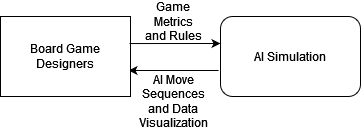
\includegraphics[width=1.0\textwidth]{System_context.png}
\caption{System Context Diagram}
\label{Fig_SystemContext} 
\end{center}
\end{figure}
%Architecture goes here of whole system base one created by prof
\newpage
\subsection{Component Diagram}
\begin{figure}[h!]
\begin{center}
 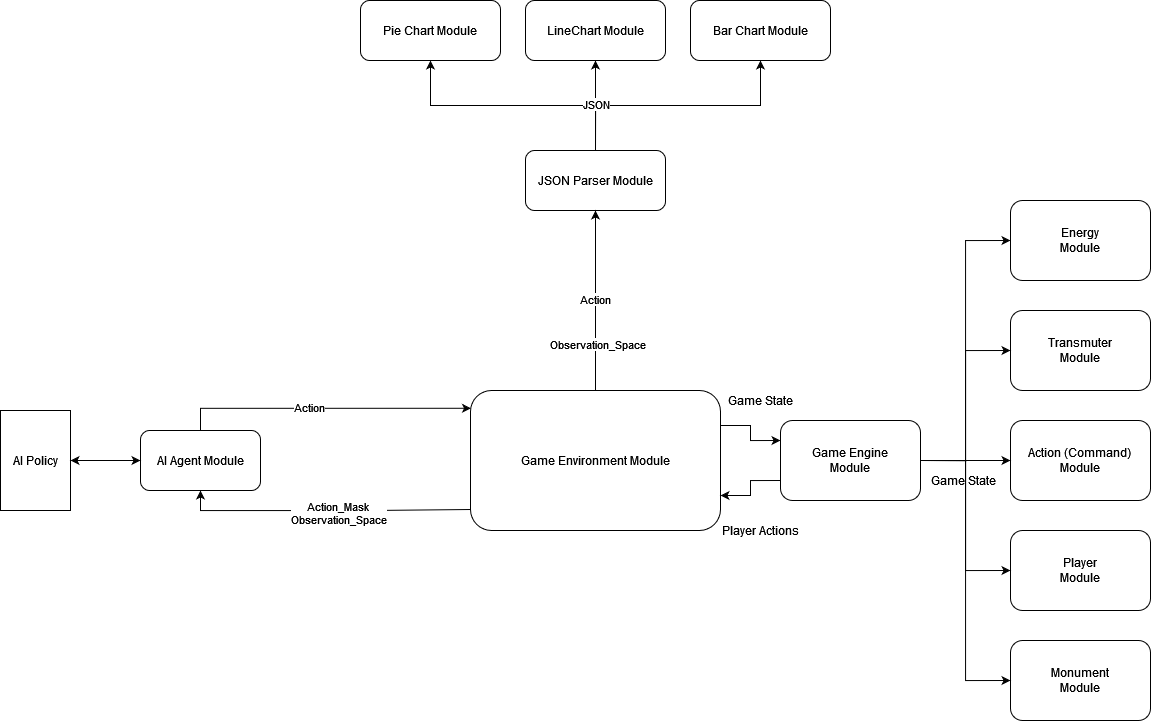
\includegraphics[width=1.0\textwidth]{Component_diagram.png}
\caption{Component Diagram}
\label{Fig_SystemContext} 
\end{center}
\end{figure}
%Game engine and smaller module breakup of architecture goes here
\newpage

\section{System Variables and Notation}
\subsection{Monitored Variables}
Monitored variables will be any variables that are observed by the system that change due to the controlled variables.


\subsection{Controlled Variables}
Controlled variables will be any variables that are controlled by the system to change the monitored variables. Refer to the output in each modules for the controlled variables. 

\subsection{Constants}
There are no constants.

\subsection{Notation}

\begin{table}[!h]
\begin{tabular}{|l|l|}
\hline
Type               & Description                                        \\ \hline
$\mathbb{N}$  & \begin{tabular}[c]{@{}l@{}}Real Numbers $\geq 0$  \end{tabular}   \\ \hline
String & \begin{tabular}[c]{@{}l@{}}sequence of characters\end{tabular}   \\ \hline
List$\langle Type \rangle$ & \begin{tabular}[c]{@{}l@{}}An array or list of the specified type\end{tabular}   \\ \hline
\textit{Object}& \begin{tabular}[c]{@{}l@{}}An instansiation of a module or abstract data type.\end{tabular}   \\ \hline
\end{tabular}
\end{table}


\newpage
\section{Module Traceability}
\begin{table}[h!]
\centering
\begin{tabular}{p{0.3\textwidth} p{0.6\textwidth}}
\toprule
\textbf{Module Name} & \textbf{Requirements}\\
\midrule

\multirow{1}{0.4\textwidth}{AI Agent Module} & FR1 FR2 FR4 FR6 NFR1 NFR3 NFR4 NFR5\\
\multirow{1}{0.4\textwidth}{Game Environment Module} & FR3 FR5 NFR1 NFR3 NFR5\\
\midrule
\multirow{1}{0.4\textwidth}{Action (Command) Module} & FR4 FR7 FR11 NFR3 NFR6\\
\multirow{1}{0.4\textwidth}{Transmuter Module} & FR10 \\
\multirow{1}{0.4\textwidth}{Monument Module} & FR10 \\
\multirow{1}{0.4\textwidth}{Energy Module} & FR10 \\
\multirow{1}{0.4\textwidth}{Player Module} & FR10 \\
\multirow{1}{0.4\textwidth}{Game Engine Module} & FR7 FR8 FR9 FR11 NFR1 NFR3 NFR4 NFR5 NFR6\\
\midrule

\multirow{1}{0.4\textwidth}{JSON Module} & FR3 FR13 NFR3\\
\multirow{1}{0.4\textwidth}{Pie Chart Module} & FR12 NFR2 NFR7\\
\multirow{1}{0.4\textwidth}{Bar Chart Module} & FR12 NFR2 NFR7\\
\multirow{1}{0.4\textwidth}{Line Chart Module} & FR12 NFR2 NFR7\\
\multirow{1}{0.4\textwidth}{JSONDataParser Module} & FR13 FR14 FR15\\
\bottomrule

\end{tabular}
\caption{Module Traceability}
\label{TblMH}
\end{table}

\newpage
\section{Abstract Data Types}
\subsection{TransmuterTile}
\subsubsection{Inputs}
\begin{table}[!h]
\begin{tabular}{|l|l|l|}
\hline
\textbf{Name}               & \textbf{Value Type}       & \textbf{Description}                                        \\ \hline
Top\_Size         & $\mathbb{N}$ & \begin{tabular}[c]{@{}l@{}}This value corresponds to the number of Energy \\ sections in top half of the tile. \end{tabular}   \\ \hline
Bottom\_Size         & $\mathbb{N}$  & \begin{tabular}[c]{@{}l@{}}This value corresponds to the number of Energy \\ sections in bottom half of the tile.\end{tabular}   \\ \hline

\end{tabular}
\end{table}

\subsubsection{Outputs}
\begin{table}[!h]
\begin{tabular}{|l|l|l|}
\hline
\textbf{Name}               & \textbf{Value Type}       & \textbf{Description}  \\ \hline
TransmuterTile  & \textit{Object} TransmuterTile & \begin{tabular}[c]{@{}l@{}} Initialized instance of a TransmuterTile type with \\ the specified input parameters\end{tabular} \\ \hline

\end{tabular}
\end{table}
\subsubsection{Description of Behaviour}
This data type is a representation of the Transmuter Tile on the player's transmuter board. It contains a method to fill the tile with an energy at a specified position on the tile and a method to empty all the energy placed on the tile. The input is used to determine the size of the top and bottom half of the tile where the energy can be placed. 

\subsubsection{Exception Handling}
Input validation will occur at the beginning of the module initialization to handle exceptions to see if any violations occur (e.g. out of bounds error). Error handling will also be done in the methods to fill a position in the tile to validate the position index and Energy type. 

\subsubsection{Initialization}
Multiple TransmuterTiles will be initialized in the Transmuter module. 

\newpage
\subsection{MonumentWall}
\subsubsection{Inputs}
\begin{table}[!h]
\begin{tabular}{|l|l|l|}
\hline
\textbf{Name}               & \textbf{Value Type}       & \textbf{Description}                                        \\ \hline
Acceptable\_Energies         & List$\langle Energy \rangle$  & \begin{tabular}[c]{@{}l@{}}As each wall can accept different energy types, \\ it is necessary to input the acceptable energy \\ types for a wall  \end{tabular}   \\ \hline
%not sure whether to add this
Benefit\_Token         & String & \begin{tabular}[c]{@{}l@{}}Once a wall is completed, the wall owner will \\ receive this benefit token allowing for special abilities.\end{tabular}   \\ \hline

\end{tabular}
\end{table}

\subsubsection{Outputs}
\begin{table}[!h]
\begin{tabular}{|l|l|l|}
\hline
\textbf{Name}               & \textbf{Value Type}       & \textbf{Description}   \\ \hline
MonumentWall  & \textit{Object} MonumentWall & \begin{tabular}[c]{@{}l@{}} Initialized instance of a MonumentWall type \\ with the specified input parameters\end{tabular} \\ \hline
\end{tabular}
\end{table}

\subsubsection{Description of Behaviour}
This data type is a representation of the Monument Wall tile on the game board. It has methods to fill an energy section and attributes to store the acceptable energy types, the current state of the wall (completed/not completed) and the benefit token. Once the energies are filled, an owner (player) will be assigned to the tile which will be useful for calculating the score at the end of the game. 

\subsubsection{Exception Handling}
Input validation will occur at the beginning of the module initialization to handle exceptions to see if any violations occur (e.g. out of bounds error, type error). Error handling will be done in methods to fill a wall section to validate the input Energy type and position index as well as if the wall hasn't already been filled. 

\subsubsection{Initialization}
Multiple MonumentWalls will be initialized in the Game Environment module. 

\newpage
\section{Module Guide}
\subsection{AI Agent Module}
\subsubsection{Inputs}
\begin{table}[!h]
\begin{tabular}{|l|l|l|}
\hline
Input Name & Input Type & Description                    \\ \hline
Epoch & $\mathbb{N}$ & \begin{tabular}[c]{@{}l@{}} Number of epochs to run.\end{tabular}   \\ \hline
Batch\_Size & $\mathbb{N}$ & \begin{tabular}[c]{@{}l@{}} Size of batch per epoch\end{tabular}   \\ \hline
Resume\_Path & String & \begin{tabular}[c]{@{}l@{}} Path to policy for the main agent. (This is the agent that \\ the policy generated will be modeled from)\end{tabular}   \\ \hline
Opponent\_Path & List$\langle String \rangle$ & \begin{tabular}[c]{@{}l@{}} Path to the policies for each of the opponents \end{tabular}   \\ \hline
Gamma & Float & \begin{tabular}[c]{@{}l@{}} Learning rate (smaller gamma, the AI will try to win earlier) \end{tabular}   \\ \hline
Agent\_Id & $\mathbb{N}$ & \begin{tabular}[c]{@{}l@{}} The ID to set for the main agent  \end{tabular}   \\ \hline
\end{tabular}
\end{table}
\subsubsection{Outputs}
\begin{table}[!h]
\begin{tabular}{|l|l|l|}
\hline
Output Name & Output Type & Description \\ \hline
Policy & $\mathbb{N}*\mathbb{N}$  & \begin{tabular}[c]{@{}l@{}} Internal filetype of AI library that stores the policy of a \\ training simulation. $\mathbb{N}$ will vary depending \\on Observation\_Space and Action\_Space \end{tabular}   \\ \hline

\end{tabular}
\end{table}

\subsubsection{Description of Behaviour}
This module will be the initial entry point into the system. After entering the inputs the module will initialize the AI Agents and their respective policies and the $\bold{Game Environment}$, that the AI Agents will interact with. The module will map the policies using the Resume\_Path for the Agent with the Id from Agent\_Id, and map the rest with the Opponent\_Path policies. Once the AI Agents and environment is ready the training will run for Epoch simulations, and during each simulation the game will be run equal to the Batch\_Size. In total the number of individual games run will be Epoch$*$Batch\_Size. Once the training is complete the module will generate a policy based off these simulations and run an additional time rendering the game simulation for the user to view the AI Agent's make decisions.
\subsubsection{Exception Handling}
Input validation will occur at the beginning of the module initialization to handle exceptions that will terminate runtime if any violations occur (type mismatch or not within bounds). Validation will also check to ensure that the paths provided point to valid files.
\subsubsection{Initialization}
Upon starting the system the AI Agent is the first to be initialized creating the AI Agents with their corresponding policies and the game environment they will interact with.

\subsection{Game Environment Module}
\subsubsection{Inputs}
\begin{table}[!h]
\begin{tabular}{|l|l|l|}
\hline
Input Name & Input Type & Description                    \\ \hline
Agents & List$\langle String \rangle$ & \begin{tabular}[c]{@{}l@{}} List of agent names \end{tabular}   \\ \hline
Action & $\mathbb{N}$ & \begin{tabular}[c]{@{}l@{}} An array index that corresponds to the action that the \\ current AI Agent will play.\end{tabular}   \\ 
\hline
\end{tabular}
\end{table}
\subsubsection{Outputs}
\begin{table}[!h]
\begin{tabular}{|l|l|l|}
\hline
Output Name & Output Type & Description \\ \hline
Rewards & List$\langle Float \rangle$ & \begin{tabular}[c]{@{}l@{}} The associated award for each agent during a single\\ game simulation \end{tabular}   \\ \hline
Observation\_Space & $\mathbb{N}*\mathbb{N}$ & \begin{tabular}[c]{@{}l@{}} Observable state of the game that is updated upon each \\ action taken. This is a matrix of $\mathbb{N}*\mathbb{N}$ \end{tabular}   \\ \hline
Action\_Space & $\mathbb{N}$ & \begin{tabular}[c]{@{}l@{}} An array of all possible actions that can be taken of size $\mathbb{N}$ \end{tabular}   \\ \hline
Action\_Mask & $\mathbb{N}$ & \begin{tabular}[c]{@{}l@{}} An array of all legal actions of size $\mathbb{N}$, an agent can take,\\ given a specific Observation\_Space\end{tabular} \\ \hline
\end{tabular}
\end{table}

\subsubsection{Description of Behaviour}
This module is the bridge between the AI Agents and the pure Game Engine. It will facilitate the input of an action taken by the AI and ensuring it is a legal move, while providing an observable state for policy learning. The module will hold information on each AI Agent's rewards to better choose which actions are better to take at certain game states. 
\subsubsection{Exception Handling}
Exception handling is done by the AI Game Environment library, where if an exception occurs like an illegal action is taken the simulation will terminate and a negative reward will be assigned to the AI. If the AI chooses an action that is out of bound (Action is higher than the length of the Action\_Space), the module will throw an error. If the Action\_Space is not in the same order during simulations an error will be thrown as these are needed for successful simulations. 
\subsubsection{Initialization}
This module is initialized after the AI Agents are initialized on the AI\_Agent Module and only initialized once. This module will then initialize the game engine along with the Observable\_Space, Action\_Space, and Rewards. Upon finishing a game simulation the module is reset and Rewards are then passed back to the AI\_Agent module.

\subsection{Game Engine Module}
\subsubsection{Inputs}
Game Engine has no explicit inputs to initialize it but rather it is the starting point of the all business logic. It is initialized to initialize the rest of the system. However, it has many dependencies on other modules to initialize them and to enforce the core business logic of the system. It uses the following modules explicitly:
\begin{itemize}
    \item Player Module
    \item Monument Module
    \item Transmuter Module
    \item EnergyTile Module
    \item ActionInitiater Module
\end{itemize}

\subsubsection{Outputs}
\begin{table}[!h]
\begin{tabular}{|l|l|l|}
\hline
Output Name & Output Type & Description \\ \hline
Engine & \textit{Object} Game Engine & \begin{tabular}[c]{@{}l@{}} Initialized instance of a Game Engine module.\\ Drives the business logic and the entry point to the game. \end{tabular}   \\ \hline
\end{tabular}
\end{table}

\subsubsection{Description of Behaviour}
This module is where the entire business logic is written and it is the entry point to the game. It uses many of the core modules of the system to initialize a new game engine and start a new simulation. Than interfacing with the Game Environment module, it provides the current state of the game and possible actions to the AI Agents and processes their response to drive the game. It also dictates the turn order of the players and keeps track of game termination conditions.

\subsubsection{Exception Handling}
There are many exception handling logic embedded inside the Game Engine module to ensure that the Player Module, Monument Module, Transmuter Module, EnergyTile Module and other aspects of the game is initialized correctly and throughout the game they are following the correct business logic. However, after initialization, if there is an error occurred, since the current simulation is not mission critical and we can gather the same data the in the next simulation, if the error handling cannot handle it and requires a human intervention, since the AI Agents won't be able to fix the issue, the data will be discarded and a new simulation will be started. This ensure the data collected is always reliable instead of trying to handle some complex errors based on the 40+ pages of game rules (business logic).

\subsubsection{Initialization}
This module is initialized when the user of the system first enters the command to run the system to the terminal. There is a \_\_main\_\_.py file that defines the entry point of the system which directly calls the Game Engine module to initialize it.

\newpage
\subsection{Player Module}
\subsubsection{Inputs}
\begin{table}[!h]
\begin{tabular}{|l|l|l|}
\hline
\textbf{Name}               & \textbf{Value Type}       & \textbf{Description}                                        \\ \hline
Character         & String  & \begin{tabular}[c]{@{}l@{}}Name of Character  \end{tabular}   \\ \hline
Agent\_Id        &  $\mathbb{N}$ & \begin{tabular}[c]{@{}l@{}} The ID to set for the main agent\end{tabular}   \\ \hline
Energies       &  List$\langle EnergyTile \rangle$  & \begin{tabular}[c]{@{}l@{}} The list of EnergyTiles that a \\ Player starts with \end{tabular}   \\ \hline

\end{tabular}
\end{table}

\subsubsection{Outputs}
\begin{table}[!h]
\begin{tabular}{|l|l|l|}
\hline
\textbf{Name}               & \textbf{Value Type}       & \textbf{Description}   \\ \hline
Player  & \textit{Object} Player & \begin{tabular}[c]{@{}l@{}} Initialized instance of a Player module with the \\specified input parameters\end{tabular} \\ \hline

\end{tabular}
\end{table}

\subsubsection{Description of Behaviour}
This module contains attributes and methods that will be used to represent a Player. At initialization, an instance of Transmuter will also be initialized. It will contain methods that will support updating the Transmuter and its TransmuterTiles. This module will also store the special abilites that a player will have based on the character name provided. It will also allow the Player to add and remove EnergyTiles in the Energies attribute.

\subsubsection{Exception Handling}
Exception handling will be done during initialization of the Player to validate the character name, list of EnergyTiles, and Agent\_Id. Additionally, any mutator methods will also have error handling to validate the input parameters and will throw the appropriate error. 

\subsubsection{Initialization}
A Player will be initialized in the AI Agent module with the required input parameters. 

\newpage
\subsection{Transmuter Module} 
\subsubsection{Inputs}
No inputs for this module.

\subsubsection{Outputs}
\begin{table}[!h]
\begin{tabular}{|l|l|l|}
\hline
\textbf{Name}               & \textbf{Value Type}       & \textbf{Description}                                        \\ \hline
Transmuter  & \textit{Object} Transmuter & \begin{tabular}[c]{@{}l@{}} Initialized instance of a Transmuter module with the \\specified input parameters\end{tabular} \\ \hline
Active\_Tiles         & List$\langle TransmuterTile \rangle$  & \begin{tabular}[c]{@{}l@{}}List of TransmuterTiles that are currently \\ on the Transmuter  \end{tabular}   \\ \hline
Reserved\_Tiles        & List$\langle TransmuterTile \rangle$ & \begin{tabular}[c]{@{}l@{}}List of TransmuterTiles that are currently \\ on reserve.\end{tabular}   \\ \hline
Action\_Tokens      & List$\langle String \rangle$ & \begin{tabular}[c]{@{}l@{}} List of tokens that corresponds with \\ a position on the Active\_Tiles. \\ Tokens represent a special ability.\end{tabular}   \\ \hline

\end{tabular}
\end{table}

\subsubsection{Description of Behaviour}
This module contains attributes and methods to represent a player's Transmuter board. As all players have the same starting TransumterTiles, there is no input for this module. The Transmuter behaves like a queue as it contains methods to convey the Active\_Tiles which removes the last active TransmuterTile and adds a TransmuterTile from the Reserved\_Tiles list to the Active\_Tiles. It will also contain methods to add, retrieve and update the Action\_Token at a particular index on the Transmuter.

\subsubsection{Exception Handling}
Exception handling will be done in methods that require inputs that will alter the state variables. Errors will be thrown if the input is in an unexpected format or if the input is invalid (e.g. list index out of bounds). Getter methods will not require any exception handling. 

\subsubsection{Initialization}
Upon initializing a Player, a Transmuter will be initialized as well.

\newpage
\subsection{Monument Module}
\subsubsection{Inputs}
\begin{table}[!h]
\begin{tabular}{|l|l|l|}
\hline
\textbf{Name}               & \textbf{Value Type}       & \textbf{Description}                                         \\ \hline
Monument\_Walls         & List$\langle MonumentWall \rangle$  & \begin{tabular}[c]{@{}l@{}}List of MonumentWalls that are on \\ on the Monument  \end{tabular}   \\ \hline
Name        & String & \begin{tabular}[c]{@{}l@{}}Name of the Monument.\end{tabular}   \\ \hline

\end{tabular}
\end{table}

\subsubsection{Outputs}
\begin{table}[!h]
\begin{tabular}{|l|l|l|}
\hline
\textbf{Name}               & \textbf{Value Type}       & \textbf{Description}  
\\ \hline
Monument  & \textit{Object} Monument & \begin{tabular}[c]{@{}l@{}} Initialized instance of a Monument module with the \\specified input parameters\end{tabular} \\ \hline
Top\_Wall\_Index         & $\mathbb{N}$   & \begin{tabular}[c]{@{}l@{}}Index of the top MonumentWall \\ on the Transmuter  \end{tabular}   \\ \hline
Completed\_Tiles        & List$\langle MonumentWalls \rangle$ & \begin{tabular}[c]{@{}l@{}}List of TransmuterTiles that are currently \\ on reserve.\end{tabular}   \\ \hline

\end{tabular}
\end{table}

\subsubsection{Description of Behaviour}
This module contains methods and attributes that represent a Monument. As each Monument can have different variations of MonumentWalls, a list of MonumentWalls is given as input to this module. It has methods to change, update and retrieve the current top MonumentWall, in accordance with the game rules. As the MonumentWalls get completed, they get added to the Completed\_Tiles output list.

\subsubsection{Exception Handling}
Exception Handling will be done during the initialization of the module to validate the input. It is necessary that the Monument\_Walls is of List$\langle MonumentWall \rangle$ type. If the type is incorrect or if the size of the list is incorrect, an error will be thrown.

\subsubsection{Initialization}
Upon starting the Game Engine, multiple Monuments will be initialized, in accordance with the game rules. 

\newpage
\subsection{EnergyTile Module}
\subsubsection{Inputs}
\begin{table}[!h]
\begin{tabular}{|l|l|l|}
\hline
\textbf{Name}               & \textbf{Value Type}       & \textbf{Description}  \\ \hline
Energy\_Type & Enum & \begin{tabular}[c]{@{}l@{}} Type of the energy which is enumerated and as \\follows:  [Constructive: 1, Invertible: 2, Generative: 3, Primal: 4] \end{tabular} \\\hline
Owner  & Player & \begin{tabular}[c]{@{}l@{}} Player which owns the energy. Each energy tile \\can only have one owner. \end{tabular}\\ \hline

\end{tabular}
\end{table}

\subsubsection{Outputs}
\begin{table}[!h]
\begin{tabular}{|l|l|l|}
\hline
\textbf{Name}               & \textbf{Value Type}       & \textbf{Description}   \\ \hline
EnergyTile  & \textit{Object} EnergyTile & \begin{tabular}[c]{@{}l@{}} Initialized instance of a EnergyTile module with one of the\\ accepted energy types \end{tabular} \\ \hline

\end{tabular}
\end{table}

\subsubsection{Description of Behaviour}
This module contains methods and attributes that represent Energy in the game. There are 4 different types of energies [Constructive: 1, Invertible: 2, Generative: 3, Primal: 4] and they are enumerated to be used throughout the system. Each energy type has different uses in the game but Primal energy type is a special one which can be used in place of other three energy types. Each energy also needs to belong to a player which is being monitored via owner variable. Methods are only getters which returns back the energy type and the owner of the energy.

\subsubsection{Exception Handling}
If the given energy type is not in the enumerated list of correct energy types, exception handling will kick in and print an error message as well as setting the energy type as invalid which would prevent it to be used during the game.

\subsubsection{Initialization}
When initialized, EnergyTile module will return an instance of EnergyTile to be used by players to make decisions and take actions based on the game rules. 

\newpage
\subsection{Command Module}
\subsubsection{Inputs}
\begin{table}[!h]
\begin{tabular}{|l|l|l|}
\hline
\textbf{Name}               & \textbf{Value Type}       & \textbf{Description}  \\ \hline
Player & Player & \begin{tabular}[c]{@{}l@{}} Player object which will use the actions that inherits command class. \end{tabular} \\\hline
Engine  & Engine & \begin{tabular}[c]{@{}l@{}} Engine object which models the game board and game rules.\end{tabular}\\ \hline

\end{tabular}
\end{table}

\subsubsection{Outputs}
\begin{table}[!h]
\begin{tabular}{|l|l|l|}
\hline
\textbf{Name}               & \textbf{Value Type}       & \textbf{Description}  \\ \hline
Command  & \textit{Object} Command & \begin{tabular}[c]{@{}l@{}} Initialized instance of a command object. \end{tabular} \\ \hline

\end{tabular}
\end{table}

\subsubsection{Description of Behaviour}
This module is a parent class to all action classes. It is named Command because it is the parent class that helps the system to implement the Command Design Pattern.

\subsubsection{Exception Handling}
N/A

\subsubsection{Initialization}
Command class and all of its sub-classes are given arguments of player and engine and automatically initialized in the ActionInitiater module (see ActionInitiater module for more details).

\newpage
\subsection{ActionTurn Module inherits Command Module}
\subsubsection{Inputs}
\begin{table}[!h]
\begin{tabular}{|l|l|l|}
\hline
\textbf{Name}               & \textbf{Value Type}       & \textbf{Description}  \\ \hline
Player & Player & \begin{tabular}[c]{@{}l@{}} Player object which will use the actions that inherits command class. \end{tabular} \\\hline
Engine  & Engine & \begin{tabular}[c]{@{}l@{}} Engine object which models the game board and game rules.\end{tabular}\\ \hline

\end{tabular}
\end{table}

\subsubsection{Outputs}
\begin{table}[!h]
\begin{tabular}{|l|l|l|}
\hline
\textbf{Name}               & \textbf{Value Type}       & \textbf{Description}   \\ \hline
ActionTurn  & \textit{Object} Command & \begin{tabular}[c]{@{}l@{}} Initialized instance of a command object.\\ Allows users to select the turn type as action turn.\end{tabular} \\ \hline
Execute  & None & \begin{tabular}[c]{@{}l@{}} Executes the action when the AI agent selects\\ this action from the action list.\end{tabular} \\ \hline
Check  & Boolean & \begin{tabular}[c]{@{}l@{}} Checks whether the action is a legal action \\ for the current player given the game state.\end{tabular} \\ \hline

\end{tabular}
\end{table}

\subsubsection{Description of Behaviour}
This module is a child class of Command class. It allows the current player to select the turn to be action turn instead of the convey turn.

\subsubsection{Exception Handling}
Exception handling is done by the check function. If the move is illegal, AI agent will receive False and won't be able to execute the action in the first place.

\subsubsection{Initialization}
Command class and all of its sub-classes are given arguments of player and engine and automatically initialized in the ActionInitiater module (see ActionInitiater module for more details).

\newpage
\subsection{ConveyTurn Module inherits Command Module}
\subsubsection{Inputs}
\begin{table}[!h]
\begin{tabular}{|l|l|l|}
\hline
\textbf{Name}               & \textbf{Value Type}       & \textbf{Description}  \\ \hline
Player & Player & \begin{tabular}[c]{@{}l@{}} Player object which will use the actions that inherits command class. \end{tabular} \\\hline
Engine  & Engine & \begin{tabular}[c]{@{}l@{}} Engine object which models the game board and game rules.\end{tabular}\\ \hline

\end{tabular}
\end{table}

\subsubsection{Outputs}
\begin{table}[!h]
\begin{tabular}{|l|l|l|}
\hline
\textbf{Name}               & \textbf{Value Type}       & \textbf{Description}   \\ \hline
ConveyTurn  & \textit{Object} Command & \begin{tabular}[c]{@{}l@{}} Initialized instance of a command object.\\ Allows users to select the turn type as convey turn.\end{tabular} \\ \hline
Execute  & None & \begin{tabular}[c]{@{}l@{}} Executes the action when the AI agent selects\\ this action from the action list.\end{tabular} \\ \hline
Check  & Boolean & \begin{tabular}[c]{@{}l@{}} Checks whether the action is a legal action \\ for the current player given the game state.\end{tabular} \\ \hline

\end{tabular}
\end{table}

\subsubsection{Description of Behaviour}
This module is a child class of Command class. It allows the current player to select the turn to be convey turn instead of the action turn.

\subsubsection{Exception Handling}
Exception handling is done by the check function. If the move is illegal, AI agent will receive False and won't be able to execute the action in the first place.

\subsubsection{Initialization}
Command class and all of its sub-classes are given arguments of player and engine and automatically initialized in the ActionInitiater module (see ActionInitiater module for more details).

\newpage
\subsection{EndTurn Module inherits Command Module}
\subsubsection{Inputs}
\begin{table}[!h]
\begin{tabular}{|l|l|l|}
\hline
\textbf{Name}               & \textbf{Value Type}       & \textbf{Description}  \\ \hline
Player & Player & \begin{tabular}[c]{@{}l@{}} Player object which will use the actions that inherits command class. \end{tabular} \\\hline
Engine  & Engine & \begin{tabular}[c]{@{}l@{}} Engine object which models the game board and game rules.\end{tabular}\\ \hline

\end{tabular}
\end{table}

\subsubsection{Outputs}
\begin{table}[!h]
\begin{tabular}{|l|l|l|}
\hline
\textbf{Name}               & \textbf{Value Type}       & \textbf{Description}   \\ \hline
EndTurn  & \textit{Object} Command & \begin{tabular}[c]{@{}l@{}} Initialized instance of a command object.\\ Allows users to end their turn.\end{tabular} \\ \hline
Execute  & None & \begin{tabular}[c]{@{}l@{}} Executes the action when the AI agent selects\\ this action from the action list.\end{tabular} \\ \hline
Check  & Boolean & \begin{tabular}[c]{@{}l@{}} Checks whether the action is a legal action \\ for the current player given the game state.\end{tabular} \\ \hline

\end{tabular}
\end{table}

\subsubsection{Description of Behaviour}
This module is a child class of Command class. It allows the current player to end their turn.

\subsubsection{Exception Handling}
Exception handling is done by the check function. If the move is illegal, AI agent will receive False and won't be able to execute the action in the first place.

\subsubsection{Initialization}
Command class and all of its sub-classes are given arguments of player and engine and automatically initialized in the ActionInitiater module (see ActionInitiater module for more details).

\newpage
\subsection{ConveyOnceFirstCard Module inherits Command Module}
\subsubsection{Inputs}
\begin{table}[!h]
\begin{tabular}{|l|l|l|}
\hline
\textbf{Name}               & \textbf{Value Type}       & \textbf{Description}  \\ \hline
Player & Player & \begin{tabular}[c]{@{}l@{}} Player object which will use the actions that inherits command class. \end{tabular} \\\hline
Engine  & Engine & \begin{tabular}[c]{@{}l@{}} Engine object which models the game board and game rules.\end{tabular}\\ \hline

\end{tabular}
\end{table}

\subsubsection{Outputs}
\begin{table}[!h]
\begin{tabular}{|l|l|l|}
\hline
\textbf{Name}               & \textbf{Value Type}       & \textbf{Description}   \\ \hline
ConveyOnceFirstCard  & \textit{Object} Command & \begin{tabular}[c]{@{}l@{}} Initialized instance of a command object.\\ Allows players to convey their first extra card.\end{tabular} \\ \hline
Execute  & None & \begin{tabular}[c]{@{}l@{}} Executes the action when the AI agent selects\\ this action from the action list.\end{tabular} \\ \hline
Check  & Boolean & \begin{tabular}[c]{@{}l@{}} Checks whether the action is a legal action \\ for the current player given the game state.\end{tabular} \\ \hline

\end{tabular}
\end{table}

\subsubsection{Description of Behaviour}
This module is a child class of Command class. It allows the current player to convey their first extra card in player's transmuter.

\subsubsection{Exception Handling}
Exception handling is done by the check function. If the move is illegal, AI agent will receive False and won't be able to execute the action in the first place.

\subsubsection{Initialization}
Command class and all of its sub-classes are given arguments of player and engine and automatically initialized in the ActionInitiater module (see ActionInitiater module for more details).

\newpage
\subsection{ConveyOnceSecondCard Module inherits Command Module}
\subsubsection{Inputs}
\begin{table}[!h]
\begin{tabular}{|l|l|l|}
\hline
\textbf{Name}               & \textbf{Value Type}       & \textbf{Description} \\ \hline
Player & Player & \begin{tabular}[c]{@{}l@{}} Player object which will use the actions that inherits command class. \end{tabular} \\\hline
Engine  & Engine & \begin{tabular}[c]{@{}l@{}} Engine object which models the game board and game rules.\end{tabular}\\ \hline

\end{tabular}
\end{table}

\subsubsection{Outputs}
\begin{table}[!h]
\begin{tabular}{|l|l|l|}
\hline
\textbf{Name}               & \textbf{Value Type}       & \textbf{Description}   \\ \hline
ConveyOnceSecondCard  & \textit{Object} Command & \begin{tabular}[c]{@{}l@{}} Initialized instance of a command object.\\ Allows players to convey their second extra card.\end{tabular} \\ \hline
Execute  & None & \begin{tabular}[c]{@{}l@{}} Executes the action when the AI agent selects\\ this action from the action list.\end{tabular} \\ \hline
Check  & Boolean & \begin{tabular}[c]{@{}l@{}} Checks whether the action is a legal action \\ for the current player given the game state.\end{tabular} \\ \hline

\end{tabular}
\end{table}

\subsubsection{Description of Behaviour}
This module is a child class of Command class. It allows the current player to convey their second extra card in player's transmuter.

\subsubsection{Exception Handling}
Exception handling is done by the check function. If the move is illegal, AI agent will receive False and won't be able to execute the action in the first place.

\subsubsection{Initialization}
Command class and all of its sub-classes are given arguments of player and engine and automatically initialized in the ActionInitiater module (see ActionInitiater module for more details).

\newpage
\subsection{ConveyTwiceFirstOrder Module inherits Command Module}
\subsubsection{Inputs}
\begin{table}[!h]
\begin{tabular}{|l|l|l|}
\hline
\textbf{Name}               & \textbf{Value Type}       & \textbf{Description}  \\ \hline
Player & Player & \begin{tabular}[c]{@{}l@{}} Player object which will use the actions that inherits command class. \end{tabular} \\\hline
Engine  & Engine & \begin{tabular}[c]{@{}l@{}} Engine object which models the game board and game rules.\end{tabular}\\ \hline

\end{tabular}
\end{table}

\subsubsection{Outputs}
\begin{table}[!h]
\begin{tabular}{|l|l|l|}
\hline
\textbf{Name}               & \textbf{Value Type}       & \textbf{Description}  \\ \hline
ConveyTwiceFirstOrder  & \textit{Object} Command & \begin{tabular}[c]{@{}l@{}} Initialized instance of a command object.\\ Allows players to convey both of their extra\\ cards with the first card going in first.\end{tabular} \\ \hline
Execute  & None & \begin{tabular}[c]{@{}l@{}} Executes the action when the AI agent selects\\ this action from the action list.\end{tabular} \\ \hline
Check  & Boolean & \begin{tabular}[c]{@{}l@{}} Checks whether the action is a legal action \\ for the current player given the game state.\end{tabular} \\ \hline

\end{tabular}
\end{table}

\subsubsection{Description of Behaviour}
This module is a child class of Command class. It allows the current player to convey both of their extra cards with the first card going in first in player's transmuter.

\subsubsection{Exception Handling}
Exception handling is done by the check function. If the move is illegal, AI agent will receive False and won't be able to execute the action in the first place.

\subsubsection{Initialization}
Command class and all of its sub-classes are given arguments of player and engine and automatically initialized in the ActionInitiater module (see ActionInitiater module for more details).

\newpage
\subsection{ConveyTwiceSecondOrder Module inherits Command Module}
\subsubsection{Inputs}
\begin{table}[!h]
\begin{tabular}{|l|l|l|}
\hline
\textbf{Name}               & \textbf{Value Type}       & \textbf{Description}  \\ \hline
Player & Player & \begin{tabular}[c]{@{}l@{}} Player object which will use the actions that inherits command class. \end{tabular} \\\hline
Engine  & Engine & \begin{tabular}[c]{@{}l@{}} Engine object which models the game board and game rules.\end{tabular}\\ \hline

\end{tabular}
\end{table}

\subsubsection{Outputs}
\begin{table}[!h]
\begin{tabular}{|l|l|l|}
\hline
\textbf{Name}               & \textbf{Value Type}       & \textbf{Description}   \\ \hline
ConveyTwiceSecondOrder  & \textit{Object} Command & \begin{tabular}[c]{@{}l@{}} Initialized instance of a command object.\\ Allows players to convey both of their extra\\ cards with the second card going in first.\end{tabular} \\ \hline
Execute  & None & \begin{tabular}[c]{@{}l@{}} Executes the action when the AI agent selects\\ this action from the action list.\end{tabular} \\ \hline
Check  & Boolean & \begin{tabular}[c]{@{}l@{}} Checks whether the action is a legal action \\ for the current player given the game state.\end{tabular} \\ \hline

\end{tabular}
\end{table}

\subsubsection{Description of Behaviour}
This module is a child class of Command class. It allows the current player to convey both of their extra cards with the second card going in first in player's transmuter.

\subsubsection{Exception Handling}
Exception handling is done by the check function. If the move is illegal, AI agent will receive False and won't be able to execute the action in the first place.

\subsubsection{Initialization}
Command class and all of its sub-classes are given arguments of player and engine and automatically initialized in the ActionInitiater module (see ActionInitiater module for more details).

\newpage
\subsection{FillMonumentWithConstructiveEnergy Module inherits Command Module}
\subsubsection{Inputs}
\begin{table}[!h]
\begin{tabular}{|l|l|l|}
\hline
\textbf{Name}               & \textbf{Value Type}       & \textbf{Description}  \\ \hline
Player & Player & \begin{tabular}[c]{@{}l@{}} Player object which will use the actions that inherits command class. \end{tabular} \\\hline
Engine  & Engine & \begin{tabular}[c]{@{}l@{}} Engine object which models the game board and game rules.\end{tabular}\\ \hline

\end{tabular}
\end{table}

\subsubsection{Outputs}
\begin{table}[!h]
\begin{tabular}{|l|l|l|}
\hline
\textbf{Name}               & \textbf{Value Type}       & \textbf{Description}   \\ \hline
FillMonumentWithConstructiveEnergy  & \textit{Object} Command & \begin{tabular}[c]{@{}l@{}} Initialized instance of a\\ command object. Allows players to fill\\ the first available monument wall\\ section with constructive energy type. \end{tabular} \\ \hline
Execute  & None & \begin{tabular}[c]{@{}l@{}} Executes the action when the AI agent\\ selects this action from the action list.\end{tabular} \\ \hline
Check  & Boolean & \begin{tabular}[c]{@{}l@{}} Checks whether the action is a\\ legal action for the current player given\\ the game state.\end{tabular} \\ \hline

\end{tabular}
\end{table}

\subsubsection{Description of Behaviour}
This module is a child class of Command class. It allows the current player to fill the first available monument wall section with constructive energy type. If the player does not have the energy type available in his hand or the section is already filled or not accepting the particular energy type, check function would already catch that and won't allow player to execute this particular action.

\subsubsection{Exception Handling}
Exception handling is done by the check function. If the move is illegal, AI agent will receive False and won't be able to execute the action in the first place.

\subsubsection{Initialization}
Command class and all of its sub-classes are given arguments of player and engine and automatically initialized in the ActionInitiater module (see ActionInitiater module for more details).

\newpage
\subsection{FillMonumentWithInvertibleEnergy Module inherits Command Module}
\subsubsection{Inputs}
\begin{table}[!h]
\begin{tabular}{|l|l|l|}
\hline
\textbf{Name}               & \textbf{Value Type}       & \textbf{Description}  \\ \hline
Player & Player & \begin{tabular}[c]{@{}l@{}} Player object which will use the actions that inherits command class. \end{tabular} \\\hline
Engine  & Engine & \begin{tabular}[c]{@{}l@{}} Engine object which models the game board and game rules.\end{tabular}\\ \hline

\end{tabular}
\end{table}

\subsubsection{Outputs}
\begin{table}[!h]
\begin{tabular}{|l|l|l|}
\hline
\textbf{Name}               & \textbf{Value Type}       & \textbf{Description}   \\ \hline
FillMonumentWithInvertibleEnergy  & \textit{Object} Command & \begin{tabular}[c]{@{}l@{}} Initialized instance of a\\ command object. Allows players to fill\\ the first available monument wall\\ section with invertible energy type. \end{tabular} \\ \hline
Execute  & None & \begin{tabular}[c]{@{}l@{}} Executes the action when the AI agent\\ selects this action from the action list.\end{tabular} \\ \hline
Check  & Boolean & \begin{tabular}[c]{@{}l@{}} Checks whether the action is a\\ legal action for the current player given\\ the game state.\end{tabular} \\ \hline

\end{tabular}
\end{table}

\subsubsection{Description of Behaviour}
This module is a child class of Command class. It allows the current player to fill the first available monument wall section with invertible energy type. If the player does not have the energy type available in his hand or the section is already filled or not accepting the particular energy type, check function would already catch that and won't allow player to execute this particular action.

\subsubsection{Exception Handling}
Exception handling is done by the check function. If the move is illegal, AI agent will receive False and won't be able to execute the action in the first place.

\subsubsection{Initialization}
Command class and all of its sub-classes are given arguments of player and engine and automatically initialized in the ActionInitiater module (see ActionInitiater module for more details).

\newpage
\subsection{FillMonumentWithGenerativeEnergy Module inherits Command Module}
\subsubsection{Inputs}
\begin{table}[!h]
\begin{tabular}{|l|l|l|}
\hline
\textbf{Name}               & \textbf{Value Type}       & \textbf{Description}  \\ \hline
Player & Player & \begin{tabular}[c]{@{}l@{}} Player object which will use the actions that inherits command class. \end{tabular} \\\hline
Engine  & Engine & \begin{tabular}[c]{@{}l@{}} Engine object which models the game board and game rules.\end{tabular}\\ \hline

\end{tabular}
\end{table}

\subsubsection{Outputs}
\begin{table}[!h]
\begin{tabular}{|l|l|l|}
\hline
\textbf{Name}               & \textbf{Value Type}       & \textbf{Description}   \\ \hline
FillMonumentWithGenerativeEnergy  & \textit{Object} Command & \begin{tabular}[c]{@{}l@{}} Initialized instance of a\\ command object. Allows players to fill\\ the first available monument wall\\ section with generative energy type. \end{tabular} \\ \hline
Execute  & None & \begin{tabular}[c]{@{}l@{}} Executes the action when the AI agent\\ selects this action from the action list.\end{tabular} \\ \hline
Check  & Boolean & \begin{tabular}[c]{@{}l@{}} Checks whether the action is a\\ legal action for the current player given\\ the game state.\end{tabular} \\ \hline

\end{tabular}
\end{table}

\subsubsection{Description of Behaviour}
This module is a child class of Command class. It allows the current player to fill the first available monument wall section with generative energy type. If the player does not have the energy type available in his hand or the section is already filled or not accepting the particular energy type, check function would already catch that and won't allow player to execute this particular action.

\subsubsection{Exception Handling}
Exception handling is done by the check function. If the move is illegal, AI agent will receive False and won't be able to execute the action in the first place.

\subsubsection{Initialization}
Command class and all of its sub-classes are given arguments of player and engine and automatically initialized in the ActionInitiater module (see ActionInitiater module for more details).

\newpage
\subsection{FillMonumentWithPrimalEnergy Module inherits Command Module}
\subsubsection{Inputs}
\begin{table}[!h]
\begin{tabular}{|l|l|l|}
\hline
\textbf{Name}               & \textbf{Value Type}       & \textbf{Description}  \\ \hline
Player & Player & \begin{tabular}[c]{@{}l@{}} Player object which will use the actions that inherits command class. \end{tabular} \\\hline
Engine  & Engine & \begin{tabular}[c]{@{}l@{}} Engine object which models the game board and game rules.\end{tabular}\\ \hline

\end{tabular}
\end{table}

\subsubsection{Outputs}
\begin{table}[!h]
\begin{tabular}{|l|l|l|}
\hline
\textbf{Name}               & \textbf{Value Type}       & \textbf{Description}   \\ \hline
FillMonumentWithPrimalEnergy  & \textit{Object} Command & \begin{tabular}[c]{@{}l@{}} Initialized instance of a\\ command object. Allows players to fill\\ the first available monument wall\\ section with primal energy type. \end{tabular} \\ \hline
Execute  & None & \begin{tabular}[c]{@{}l@{}} Executes the action when the AI agent\\ selects this action from the action list.\end{tabular} \\ \hline
Check  & Boolean & \begin{tabular}[c]{@{}l@{}} Checks whether the action is a\\ legal action for the current player given\\ the game state.\end{tabular} \\ \hline

\end{tabular}
\end{table}

\subsubsection{Description of Behaviour}
This module is a child class of Command class. It allows the current player to fill the first available monument wall section with primal energy type. If the player does not have the energy type available in his hand or the section is already filled or not accepting the particular energy type, check function would already catch that and won't allow player to execute this particular action.

\subsubsection{Exception Handling}
Exception handling is done by the check function. If the move is illegal, AI agent will receive False and won't be able to execute the action in the first place.

\subsubsection{Initialization}
Command class and all of its sub-classes are given arguments of player and engine and automatically initialized in the ActionInitiater module (see ActionInitiater module for more details).

\newpage
\subsection{ActionInitiater Module inherits Command Module} 
\subsubsection{Inputs}
\begin{table}[!h]
\begin{tabular}{|l|l|l|}
\hline
\textbf{Name}               & \textbf{Value Type}       & \textbf{Description}  \\ \hline
Player & Player & \begin{tabular}[c]{@{}l@{}} Player object which will use the actions that inherits command class. \end{tabular} \\\hline
Engine  & Engine & \begin{tabular}[c]{@{}l@{}} Engine object which models the game board and game rules.\end{tabular}\\ \hline

\end{tabular}
\end{table}

\subsubsection{Outputs}
\begin{table}[!h]
\begin{tabular}{|l|l|l|}
\hline
\textbf{Name}               & \textbf{Value Type}       & \textbf{Description}  \\ \hline
Get\_Actions  & List$\langle Command \rangle$ & \begin{tabular}[c]{@{}l@{}} Initializes all the subclasses of Command\\ module and returns it as a list. \end{tabular} \\ \hline
\end{tabular}
\end{table}

\subsubsection{Description of Behaviour}
This module only have one function, it is static and called in the Engine module. It goes through all the modules in the src/env/actions package (subfolder) and initializes all the subclasses of the Command module and returns it as a list of actions to be used in the game engine and game environment to allow AI Agents to select useful actions by observing the action space.

\subsubsection{Exception Handling}
Exception handling is done by the python's \_\_init\_\_.py file which makes the actions folder a package where if it cannot find a file will throw an error. There is no other special error handling done by our system.

\subsubsection{Initialization}
No initialization is needed. ActionInitiater only have one function, it is static and called in the Engine module.

\newpage
\subsection{JSON Module}
\subsubsection{Inputs}
\begin{table}[!h]
\begin{tabular}{|l|l|l|}
\hline
\textbf{Name}               & \textbf{Value Type}       & \textbf{Description}                                         \\ \hline
Agent         & String  & \begin{tabular}[c]{@{}l@{}}A string representing the AI Agent that played the \\ corresponding action.  \end{tabular}   \\ \hline
Turn\_Num       & $\mathbb{N}$  & \begin{tabular}[c]{@{}l@{}}A numerical value represented the turn \\ that the action was played on.  \end{tabular}   \\ \hline
Action         & $\mathbb{N}$  & \begin{tabular}[c]{@{}l@{}}An array index that corresponds to the \\ action 
that AI Agent will play.  \end{tabular}   \\ \hline
Action\_Details        &  String & \begin{tabular}[c]{@{}l@{}} Additional details about the specified action. \end{tabular}   \\ \hline
Current\_Score       &  Float  & \begin{tabular}[c]{@{}l@{}} The current score that the agent has \\ after playing the action. \end{tabular}   \\ \hline

\end{tabular}
\end{table}

\subsubsection{Outputs}
\begin{table}[!h]
\begin{tabular}{|l|l|l|}
\hline
\textbf{Name}               & \textbf{Value Type}       & \textbf{Description}                                        \\ \hline
Simulation\_History         & JSON File  & \begin{tabular}[c]{@{}l@{}}Contains a JSON of each action taken during \\
a single game simulation along \\ with the player,
turn number and action number.  \end{tabular}   \\ \hline

\end{tabular}
\end{table}
\subsubsection{Description of Behaviour}
This module contains the attributes and  methods used to gather the information from the simulation and then store them in a JSON file for further use in other modules.

\subsubsection{Exception Handling}
Exception handling will be done during the reading and writing of the JSON file to validate that the correct information is being written to the right file, and no extraneous files are being created during this process. 

\subsubsection{Initialization}
The simulation history file will be initialized at the start of the simulation, in which the history be constantly updated as each move is made by the AI agents in the simulation.


\newpage
\subsection{JSONDataParser Module}
\subsubsection{Inputs}
\begin{table}[!h]
\begin{tabular}{|l|l|l|}
\hline
\textbf{Name}               & \textbf{Value Type}       & \textbf{Description}                                        \\ \hline
jsonFile         & String  & \begin{tabular}[c]{@{}l@{}} Path of the JSON File  \end{tabular}   \\ \hline

\end{tabular}
\end{table}

\subsubsection{Outputs}
\begin{table}[!h]
\begin{tabular}{|l|l|l|}
\hline
\textbf{Name}               & \textbf{Value Type}       & \textbf{Description}                                         \\ \hline
jsonData         & JSON Object  & \begin{tabular}[c]{@{}l@{}}JSON data object fetched from JSON File
  \end{tabular}   \\ \hline

\end{tabular}
\end{table}
\subsubsection{Description of Behaviour}
This module is the bridge between Game Engine and Data Visualization model. It will effectively help the Data Visualization model fetch data from the JSON log file in Game Engine. 

\subsubsection{Exception Handling}
Exception handling will be done during the initialization of the JSONDataParser to validate the jsonFile. Errors will be thrown if the jsonFile path is invalid or the content in the jsonFile is not in JSON format. 

\subsubsection{Initialization}
A JSONDataParser will be initialized after the JSON log file is generated from the game engine. 


\newpage
\subsection{PieChart Module}
\subsubsection{Inputs}
\begin{table}[!h]
\begin{tabular}{|l|l|l|}
\hline
\textbf{Name}               & \textbf{Value Type}       & \textbf{Description}                                        \\ \hline
jsonInput         &  JSON Object  & \begin{tabular}[c]{@{}l@{}} JSON data fetched from the log file  \end{tabular}   \\ \hline
edgecolor         &  String   & \begin{tabular}[c]{@{}l@{}} Edge color that separates different wedges of the piechart   \end{tabular}   \\ \hline 
chartTitle         &   String  & \begin{tabular}[c]{@{}l@{}} Title of the pie chart  \end{tabular} \\ \hline
pngTargetDirectory         &  String  & \begin{tabular}[c]{@{}l@{}} The file path of the expected pie chart png output  \end{tabular} \\ \hline
objectName         &  String  & \begin{tabular}[c]{@{}l@{}} The object that uses for pie chart statistic calculation  \end{tabular} \\ \hline

\end{tabular}
\end{table}

\subsubsection{Outputs}
\begin{table}[!h]
\begin{tabular}{|l|l|l|}
\hline
\textbf{Name}               & \textbf{Value Type}       & \textbf{Description}                                         \\ \hline
pieChartPNG          & png file  & \begin{tabular}[c]{@{}l@{}}Pie Chart model in png file format
  \end{tabular}   \\ \hline

\end{tabular}
\end{table}
\subsubsection{Description of Behaviour}
This module contains attributes and methods that will be used to define the statistical information of the Pie Chart. It has methods to retrieve, change, and assign the statistic input and the characteristics of the Pie Chart. After the PieChart object  is initialized, it will generate a pie Chart model in the target directory.  

\subsubsection{Exception Handling}
The Exception handling will be done during the initialization of PieChart to validate the input. Errors will be thrown if the statistic objectName and pngTargetDirectory are invalid. 


\subsubsection{Initialization}
A PieChart object will be initialized after inputting appropriate jsonInput, objectName, and pngTargetDirectory. 


\newpage
\subsection{BarChart Module}
\subsubsection{Inputs}
\begin{table}[!h]
\begin{tabular}{|l|l|l|}
\hline
\textbf{Name}               & \textbf{Value Type}       & \textbf{Description}                                       \\ \hline
jsonInput         &  JSON Object  & \begin{tabular}[c]{@{}l@{}} JSON data fetched from the log file  \end{tabular}   \\ \hline 
chartTitle         &   String  & \begin{tabular}[c]{@{}l@{}} Title of the bar chart  \end{tabular} \\ \hline
pngTargetDirectory         &  String  & \begin{tabular}[c]{@{}l@{}} The file path of the expected bar chart png output  \end{tabular} \\ \hline
objectName         &  String  & \begin{tabular}[c]{@{}l@{}} The object that uses for bar chart statistic calculation  \end{tabular} \\ \hline

\end{tabular}
\end{table}

\subsubsection{Outputs}
\begin{table}[!h]
\begin{tabular}{|l|l|l|}
\hline
\textbf{Name}               & \textbf{Value Type}       & \textbf{Description}                                        \\ \hline
BarChartPNG             & png file  & \begin{tabular}[c]{@{}l@{}}Bar Chart  model in png file format
  \end{tabular}   \\ \hline

\end{tabular}
\end{table}
\subsubsection{Description of Behaviour}
This module contains attributes and methods that will be used to define the statistical information of the Bar Chart. It has methods to retrieve, change, and assign the statistic input and display the distribution of data points in the Bar Chart. After the BarChart object is initialized, it will generate a horizontal bar chart model in the target directory.  

\subsubsection{Exception Handling}
The Exception handling will be done during the initialization of BarChart to validate the input. Errors will be thrown if the statistic objectName and pngTargetDirectory are invalid. 


\subsubsection{Initialization}
A BarChart object will be initialized after inputting the appropriate jsonInput, objectName, and pngTargetDirectory.  




\newpage
\subsection{LineChart Module}
\subsubsection{Inputs}
\begin{table}[!h]
\begin{tabular}{|l|l|l|}
\hline
\textbf{Name}               & \textbf{Value Type}       & \textbf{Description}                                        \\ \hline
jsonInput         &  JSON Object  & \begin{tabular}[c]{@{}l@{}} JSON data fetched from the log file  \end{tabular}   \\ \hline 
chartTitle         &   String  & \begin{tabular}[c]{@{}l@{}} Title of the line chart  \end{tabular} \\ \hline
pngTargetDirectory         &  String  & \begin{tabular}[c]{@{}l@{}} The file path of the expected bar chart png output  \end{tabular} \\ \hline
targetDataType         &  String  & \begin{tabular}[c]{@{}l@{}} target Object to compare  \end{tabular} \\ \hline

Players         &  List(Players)  & \begin{tabular}[c]{@{}l@{}} The list of Player objects  \end{tabular} \\ \hline

\end{tabular}
\end{table}

\subsubsection{Outputs}
\begin{table}[!h]
\begin{tabular}{|l|l|l|}
\hline
\textbf{Name}               & \textbf{Value Type}       & \textbf{Description}                                        \\ \hline
LineChartPNG             & png file  & \begin{tabular}[c]{@{}l@{}}Line Chart model in png file format
  \end{tabular}   \\ \hline

\end{tabular}
\end{table}
\subsubsection{Description of Behaviour}
This module contains attributes and methods that will be used to display the graphic information in the Line Chart. It has methods to retrieve, change, and assign the data points, show their trends and efficiently make a comparison within the Line Chart. After the LineChart object is initialized, it will generate a Line Chart model in the target directory. 

\subsubsection{Exception Handling}
The Exception handling will be done during the initialization of LineChart to validate the input. Errors will be thrown if the targetDataType, pngTargetDirectory, jsonInput, Players are invalid. 


\subsubsection{Initialization}
A LineChart object will be initialized after inputting the appropriate jsonInput, targetDataType, Players, pngTargetDirectory. 






\newpage
\section*{Appendix A}
\subsection*{Limitations of Design}
The high modularity of the design, each specific component is its own module and they communicate through a specified interface allows for each module to be developed independently. Though the limitation of this is one cannot fully test their module without integration with the other modules, specifically the AI Agent Module cannot be fully tested and approved as working until the Game Engine Modules and Game Environment Modules are completed. This leads to integration errors that take significant development time to solve. For example if a new game mechanic wants to be added, it is first added in the Game Engine Modules, this can be tested only within the game engine without any AI interaction. Only once the AI Agent and Game Engine modules are both updated can they be integrated and checked for bugs and errors, which occur mostly during runtime as the AI can explore many different edge cases which may not have been tested and covered in the initial testing of the Game Engine modules. 
Another limitation of this system is the architecture can only support turn based games as it can only accept one action for one player at a time, this means for a parallel (real-time) game the architecture will not be supported.

\subsection*{Benefits and Trade offs of Other Solutions}
Our group found that there are not any other solutions available for the system that we are developing. While standalone application of parts of our system have been created before, no one has incorporated our 3 major components of an AI, game engine and data visualization before. For example, a standalone AI game player exists like AlphaGO. Developed by Google, it is the first computer program to defeat a professional human Go player, the first to defeat a Go world champion, and is arguably the strongest Go player in history. Our system does not focus on creating the best AI player that could beat any human playing Age Contrived but rather it is an essential part in simulating multiple iterations of the game with different strategies. We found one system that incorpates the AI and game engine but lacks the data visualization that we are aiming for. Blockus Game Solver, \url{https://digitalcommons.calpoly.edu/cgi/viewcontent.cgi?article=1305&context=cpesp}, is quite similar to our system as it aims to find winning strategies and loopholes in a multiplayer game. The report outlines strategies that they found had better outcomes, however, it lacks in providing the reader with an easy and intuitive way to visualize the outcomes and does not provide the level of modularity that our system is being developed with.  

\newpage
\subsection*{Development Timeline}
Below is an estimate for module completion start and end date, the resource will be in charge of main development, but all developers will aid in architecture and integration.
\begin{table}[h!]
\scalebox{0.80}{
\begin{tabular}{|l|l|l|l|l|}
\hline
Module &
  Start Date &
  Completion Date &
  Resource &
  Description \\ \hline
AI Agent &
 11-7-2022 &
 12-11-2022 &
  Michael &
  \begin{tabular}[c]{@{}l@{}}Apart of initial MVP to setup \\ the architecture, components will \\ be highly coupled to get initial \\framework\end{tabular} \\ \hline
Game Environment &
 11-7-2022 &
 12-11-2022 &
  Michael &
  \begin{tabular}[c]{@{}l@{}}Apart of initial MVP to setup \\ the architecture, components will \\ be highly coupled to get initial \\ framework\end{tabular} \\ \hline
Game Engine &
 11-7-2022 &
 12-11-2022 &
  Michael &
  \begin{tabular}[c]{@{}l@{}}Apart of initial MVP to setup \\ the architecture, components will \\ be highly coupled to get initial \\ framework\end{tabular} \\ \hline
Transmuter &
 12-12-2022 &
 12-31-2022 &
  Hargun &
  Core game mechanic \\ \hline
Player &
 12-12-2022 &
 12-31-2022 &
  Jonah &
  Core game mechanic \\ \hline
Actions (Also named Commands) &
 1-1-2023 &
 1-22-2023 &
  Jonah &
  \begin{tabular}[c]{@{}l@{}}Decoupling to add extensibility \\to additional game mechanics \\(Architecture change)\end{tabular} \\ \hline
Monument &
 1-1-2023 &
 1-22-2023 &
  Hargun &
  Core game mechanic \\ \hline
Energy &
 1-1-2023 &
 1-22-2023 &
  Jonah &
  \begin{tabular}[c]{@{}l@{}}Decoupling to add extensibility \\to additional game mechanics \\(core mechanic)\end{tabular} \\ \hline
JSON &
 1-1-2023 &
 1-15-2023 &
  Jeffrey &
  \begin{tabular}[c]{@{}l@{}} Needed to bridge simulation \\ to data visualizer\end{tabular} \\ \hline
JSONDataParser &
 1-1-2023 &
 1-15-2023 &
  Tianzheng &
  \begin{tabular}[c]{@{}l@{}} Need to fetch the output log \\ data to data visualizer\end{tabular} \\ \hline
PieChart &
 1-1-2023 &
 1-29-2023 &
  Tianzheng &
  \begin{tabular}[c]{@{}l@{}}Visualize data to \\solve business goals, \\ can be done in parrallel \\ with other modules\end{tabular} \\ \hline
BarChart &
 1-1-2023 &
 1-29-2023 &
  Tianzheng &
  \begin{tabular}[c]{@{}l@{}}Visualize data to \\solve business goals, \\ can be done in parallel \\with other modules\end{tabular} \\ \hline
LineChart &
 1-1-2023 &
 1-29-2023 &
  Tianzheng &
  \begin{tabular}[c]{@{}l@{}}Visualize data to \\ solve business goals,\\ can be done in parallel \\ with other modules\end{tabular} \\ \hline
\end{tabular}}
\caption{Module Timeline}
\label{MTL}
\end{table}

\end{document}

